\documentclass{beamer}
\usetheme{Boadilla}
\usepackage[ngerman]{babel}
\usepackage[utf8]{inputenc}
\usepackage[T1]{fontenc}
\usepackage{lmodern}
\usepackage{hyperref}
\usepackage{listings} 
\usepackage{graphicx}
\usepackage{pgf}
\usepackage{color}
\definecolor{ex_green_titel}{RGB}{204,230,204}
\definecolor{ex_green}{RGB}{230,243,230}
\definecolor{light-gray}{gray}{0.95}

\begin{document}
\lstset{ 						%
language=bash,                % the language of the code
basicstyle=\footnotesize,       % the size of the fonts that are used for the code
numbers=right,                   % where to put the line-numbers
numberstyle=\footnotesize,      % the size of the fonts that are used for the line-numbers
stepnumber=2,                   % the step between two line-numbers. If it's 1, each line 
                                % will be numbered
numbersep=-10pt,                  % how far the line-numbers are from the code
backgroundcolor=\color{light-gray},  % choose the background color. You must add \usepackage{color}
showspaces=false,               % show spaces adding particular underscores
showstringspaces=false,         % underline spaces within strings
showtabs=false,                 % show tabs within strings adding particular underscores
frame=single,                   % adds a frame around the code
tabsize=2,                      % sets default tabsize to 2 spaces
captionpos=b,                   % sets the caption-position to bottom
breaklines=true,                % sets automatic line breaking
breakatwhitespace=false,        % sets if automatic breaks should only happen at whitespace
%title=\lstname,                 % show the filename of files included with \lstinputlisting;
                                % also try caption instead of title
escapeinside={\%*}{*)},         % if you want to add a comment within your code
morekeywords={*,...}            % if you want to add more keywords to the set
}

\title{Eine Einführung in Versionverwaltungsysteme}   
\subtitle{Wissenswertes für GIT-Anwender}
\titlegraphic{
\includegraphics[width=2cm,height=2cm]{erlangen}}
\author[Bernd Wunder]{bernd.wunder@leb.eei.uni-erlangen.de} 
\institute[LEB -- TF Uni Erlangen]{Lehrstuhl für Elektronische Bauelemente\\ Friedrich-Alexander-Universität Erlangen-Nürnberg}
\date{\today}
\logo{
\includegraphics[scale=0.08]{erlangen}}

\begin{frame}
\titlepage
\end{frame}

\begin{frame}
\frametitle{Inhaltsverzeichnis}\tableofcontents
\end{frame}


\section{Einführung} 
\subsection{Versionsverwaltungsysteme}
\begin{frame}\frametitle{Versionsverwaltungsysteme} 

\begin{quote}
Eine Versionsverwaltung ist ein System, das zur Erfassung von Änderungen an Dokumenten oder Dateien verwendet wird. Alle Versionen werden in einem Archiv mit Zeitstempel und Benutzerkennung gesichert und können später wiederhergestellt werden.
\footnote{Quelle: \href{http://de.wikipedia.org/wiki/Versionsverwaltung}{Wikipedia}}
\end{quote} 

Aufgaben
\begin{itemize}
\item  Protokollierungen der Änderungen
\item  Wiederherstellung von alten Ständen 
\item  Archivierung der einzelnen Stände eines Projektes
\item  Kooperative Entwicklung (Entwicklungsteams)
\item  gleichzeitige Entwicklung mehrerer Entwicklungszweige (branches)
\end{itemize} 
\end{frame}

\begin{frame}\frametitle{Versionsverwaltungsysteme} 

engl. Bezeichnungen: \textit{Version Control System (VCS)}, \textit{Software Configuration Management (SCM)}, \textit{Revision Control System (RCS)}

\vspace*{0.15cm}
\textbf{unvollständige Übersicht einiger VCSe:}
\begin{block}{Revision Control System (RCS)}
	\begin{tabular}{l c}
Entwicklung: & 1980 bis 2004  \\  
Einteilung: & zentrales, dateibasiertes VCS \\ 
Probleme: & Binärdateien, Verzeichnisse, locks, merge, \\
          & keine Atomic commits, keine Metadaten, umbenennen  \\
Prüfsumme: & --- \\
Compression: & --- \\
Lizenz: & GPL2 \\
Betriebsysteme: & UNIX, WIN95 \\

\end{tabular} 

\vspace*{0.3cm}
Entwickelt für die Versionsverwaltung von Text-Dateien auf einem Computer!
RCS ist im Wesentlichen mit ersten VCS, dem \textit{Source Code Control System (SCCS)}, vergleichbar.
\end{block}


\end{frame}

\begin{frame}\frametitle{Versionsverwaltungsysteme} 

\begin{block}{Concurrent Versions System (CVS)}
	\begin{tabular}{l c}
basierend auf: & RCP (nutzt gleiches Speicherformat) \\ 
Entwicklung: & 1989 bis 2008  \\  
Einteilung: & zentrales VCS \\ 
Probleme: & Binärdateien, Verzeichnisse, locks, merge, \\
          & keine Atomic commits, keine Metadaten, umbenennen  \\
Prüfsumme: & --- \\
Compression: & --- \\
Lizenz: & GPL2 \\
Betriebsysteme: & UNIX, WINDOWS, Mac OS X \\
\end{tabular} 

\vspace*{0.3cm}
CVS wird nicht mehr aktiv weiterentwickelt. Die offizielle Webseite wird nicht mehr weiter betreut. \footnote{Quelle: \href{http://de.wikipedia.org/wiki/Concurrent_Versions_System}{Wikipedia}}
\end{block}


\end{frame}

\begin{frame}\frametitle{Versionsverwaltungsysteme} 

\begin{block}{Subversion (SVN)}
	\begin{tabular}{l c}
basierend auf: & CVS (Nachfolger) \\ 
Entwicklung: & seit 2000  \\  
 & Ziele CVS Probleme (siehe oben) zu beseitigen \\
Einteilung: & zentrales VCS \\ 
Probleme: & Binärdateien, Verzeichnisse, locks, merge \\
Prüfsumme: & --- \\
Compression: & --- \\
Lizenz: & Apache License \\
Betriebsysteme: & UNIX, WINDOWS, Mac OS X \\
\end{tabular} 

\vspace*{0.3cm}
CVS wird nicht mehr aktiv weiterentwickelt. Die offizielle Webseite wird nicht mehr weiter betreut. \footnote{Quelle: \href{http://de.wikipedia.org/wiki/Concurrent_Versions_System}{Wikipedia}}
\end{block}


\end{frame}

\subsection{Grundbegriffe}
\begin{frame}\frametitle{Grundbegriffe}
\begin{block}{Repository}
Datenbank in dem jeder Dateistand eines Projektes über die Zeit hinweg gespeichert ist.
\end{block}

\begin{block}{Working Tree}
Arbeitsverzeichnis in dem die Modifikationen durchgeführt werden.
\end{block}

\begin{block}{Commit}
beinhaltet alle Veränderungen bzw. spiegelt den aktuellen Zustand der in das VCS aufgenommen werden soll wieder. Enthält neben den Änderungen zusätzliche Metadaten (Commit Message, Autor, Datum, Signatur, ...)
\end{block}

\begin{block}{HEAD}
zeigt auf die neueste Version \textit{Kopf} im aktuellen Zweig (Branch)

Achtung: Unterschide zwischen GIT und SVN,CVS
\end{block}
\end{frame}

\begin{frame}\frametitle{Grundbegriffe}
\begin{block}{Secure Hash Algorithm (SHA-1)}
ist eine eindeutige, 160 Bit (40 hexadezimale Zeichen) lange Prüfsumme für beliebige digitale Informationen.
\end{block}

\begin{exampleblock}{Beispiel:}
mit dem GNU/Linux Programm \textit{sha1sum} wird die Prüfsumme für den Text \textit{"'Isabella und Lilly Wunder"'} berechnet werden:
\lstinputlisting{bash.txt}
\end{exampleblock}

\end{frame}
\begin{frame}\frametitle{Grundbegriffe (GIT)}

\begin{block}{\textit{Branch}}
bezeichnet einen parallelen Entwicklungszweig. Der Hauptzweig in einem Versionsverwaltungssystem hat meistens einen speziellen Namen. ( z.B in SVN->\textit{trunk} und in GIT->\textit{master})
\end{block}

\begin{block}{Objektmodell}
Git-Objekte (blob, tree, commit, tag) sind in einer Objektdatenbank gespeichert und über SHA1-Summen identifizierbar. Die History eines Repository lässt sich als Graph von Objekten modellieren.
\end{block}

\begin{block}{\textit{Index}}
Der \textit{Index} ist ein lokaler Zwischenspeicher. Alle Änderungen werden zuerst in den index geschrieben. Anschießend wird der Index durch einen \textit{commit} in das Repository eingecheckt. 
\end{block}

\end{frame}
\begin{frame}\frametitle{Grundbegriffe (GIT)}

\begin{block}{\textit{Clone}}
ist eine Kopie eines Repositories mit der gesamten History der Entwicklung.
\end{block}

\begin{block}{\textit{Tag}}
Ein Tag ist ein symbolischer Name für schwer zu merkende SHA-1 Summen. So können spezielle \textit{Commit} einen Namen, also ein \textit{Tag} erhalten. 
\end{block}

\end{frame}


\section{Grundlegende Konzepte} 
\subsection{Warum Versionsverwaltung}\frametitle{Warum Versionsverwaltung}

\begin{frame}\frametitle{Warum Versionsverwaltung}
\begin{columns}
        \column{.55\textwidth}
                \pgfimage[width=\textwidth]{Bilder/chaosschreibtisch}
        \column{.45\textwidth}
                \begin{enumerate}
                \item viele gleichzeitige laufende Projekte / Features (z.B. Sicherheitsupdates, neue Funktionstests, verschiedene Versionen)
                \item Um des Chaos Herr zu werden
                \end{enumerate}
\end{columns}

\end{frame}
\begin{frame}\frametitle{Warum Versionsverwaltung}
\begin{columns}
        \column{.55\textwidth}
                \pgfimage[width=\textwidth]{Bilder/schreibtisch}
        \column{.45\textwidth}
                \begin{enumerate}
                \item viele gleichzeitige laufende Projekte / Features (z.B. Sicherheitsupdates, neue  Funktionstests, verschiedene Versionen)
                \item Um des Chaos Herr zu werden
                \item Überblick über die gesamte Entwicklung behalten
                \item kolaboratives Arbeiten in einem Team
                \end{enumerate}
\end{columns}
\end{frame}

\subsection{Branches, Merges und Tags}
\begin{frame}\frametitle{Branches, Merges und Tags}
\begin{description}
\item[Branch] Parralle Entwicklung in Teams erfordert oft mehrere Zweige
\item[Tag] Name für eine bestimmte Version 
\item[Merge] Führt den Parallelen Zweig in den Hauptzweig zurück
\item[Trunk] Name in SVN für den Hauptentwicklungszweig
\end{description}

\begin{figure}
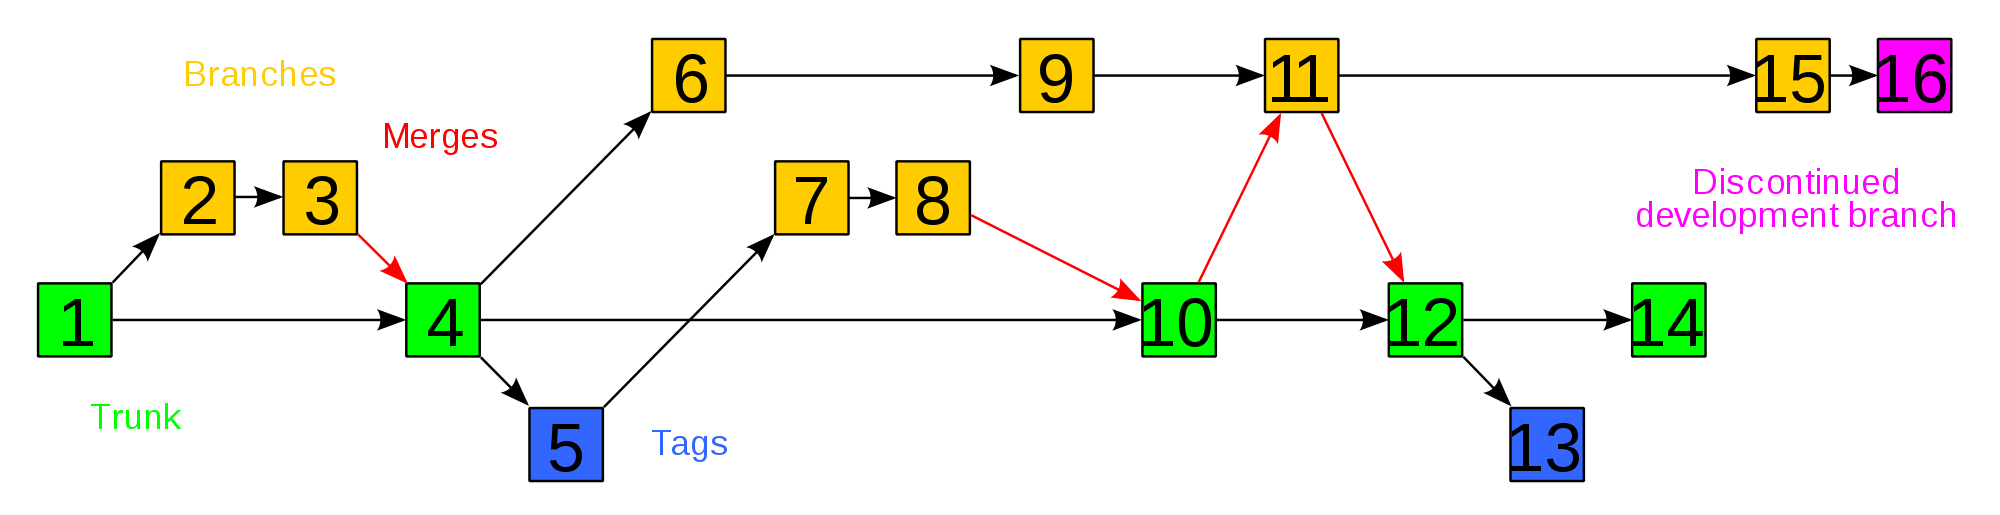
\includegraphics[scale=0.15]{2000px-Subversion_project_visualization} 
\caption{Branches, Merges und Tags \footnote{Quelle: \href{http://en.wikipedia.org/wiki/File:Subversion_project_visualization.svg}{Wikipedia}}}
\end{figure}


\end{frame}

\begin{frame}\frametitle{Aufz\"ahlung mit Pausen}
\begin{itemize}
\item  Einf\"uhrungskurs in \LaTeX \pause 
\item  Kurs 2 \pause 
\item  Seminararbeiten und Pr\"asentationen mit \LaTeX \pause 
\item  Die Beamerclass
\end{itemize} 
\end{frame}

\subsection{Zweige, Branches, ...}
\begin{frame}\frametitle{Numerierte Liste}
\begin{enumerate}
\item  Einf\"uhrungskurs in \LaTeX 
\item  Kurs 2
\item  Seminararbeiten und Pr\"asentationen mit \LaTeX 
\item  Die Beamerclass
\end{enumerate}
\end{frame}
\begin{frame}\frametitle{Numerierte Liste mit Pausen}
\begin{enumerate}
\item  Einf\"uhrungskurs in \LaTeX \pause 
\item  Kurs 2 \pause 
\item  Seminararbeiten und Pr\"asentationen mit \LaTeX \pause 
\item  Die Beamerclass
\end{enumerate}
\end{frame}

\section{Abschnitt Nr.3} 
\subsection{Tabellen}
\begin{frame}
\frametitle{Tabellen}
\begin{tabular}{|c|c|c|}
\hline
\textbf{Zeitpunkt} & \textbf{Kursleiter} & \textbf{Titel} \\
\hline
WS 04/05 & Sascha Frank &  Erste Schritte mit \LaTeX  \\
\hline
SS 05 & Sascha Frank & \LaTeX \ Kursreihe \\
\hline
\end{tabular}
\end{frame}


\begin{frame}
\frametitle{Tabellen mit Pause}
\begin{tabular}{c c c}
A & B & C \\ 
\pause 
1 & 2 & 3 \\  
\pause 
A & B & C \\ 
\end{tabular} 
\end{frame}


\section{Abschnitt Nr.4}
\subsection{Bl\"ocke}
\begin{frame}\frametitle{Bl\"ocke}

\begin{block}{Blocktitel}
Blocktext 
\end{block}

\begin{exampleblock}{Blocktitel}
Blocktext 
\end{exampleblock}


\begin{alertblock}{Blocktitel}
Blocktext 
\end{alertblock}
\end{frame}

\section[Quellen]{Referezen}
\begin{frame}\frametitle{Quellen \& Literatur}

\begin{thebibliography}{9}
\bibitem[Beamerpaket]{paket} \emph{Beamer Paket} \\ 
\text{http://latex-beamer.sourceforge.net/}
\bibitem[Beamerdokumentation]{doku} \emph{User's Guide to the Beamer} 
\bibitem[Dante]{dante} \emph{DANTE e.V.} \text{http://www.dante.de}   
\end{thebibliography}


\end{frame}



\end{document}

